\documentclass[10pt]{beamer}
\usepackage[utf8]{inputenc}
\usepackage[T1]{fontenc}
\usepackage{mathabx}
\usepackage{amsmath}
\usepackage{mathpazo}
\usepackage{eulervm}
\usepackage{ragged2e}
\usepackage{graphicx}
\usepackage{xcolor}
\usepackage{booktabs}
\usepackage{mathtools}
\usepackage{bbm}
\usepackage{animate}
\usepackage{tikz}
\usepackage{MnSymbol,wasysym}
\usepackage[sorting=ydnt,bibstyle=ieee]{biblatex}
\addbibresource{Ref.bib}
\setbeamertemplate{bibliography item}{}
\AtEveryCite{\color{blue}}
\usepackage{todonotes} % \missingfigure 
\usepackage{comment} % to exclude whole sections when I want to

\DeclareMathOperator{\E}{\mathbb{E}}

%%Implements Justified text all over.
\makeatletter
\renewcommand{\itemize}[1][]{%
  \beamer@ifempty{#1}{}{\def\beamer@defaultospec{#1}}%
  \ifnum \@itemdepth >2\relax\@toodeep\else
    \advance\@itemdepth\@ne
    \beamer@computepref\@itemdepth% sets \beameritemnestingprefix
    \usebeamerfont{itemize/enumerate \beameritemnestingprefix body}%
    \usebeamercolor[fg]{itemize/enumerate \beameritemnestingprefix body}%
    \usebeamertemplate{itemize/enumerate \beameritemnestingprefix body begin}%
    \list
      {\usebeamertemplate{itemize \beameritemnestingprefix item}}
      {\def\makelabel##1{%
          {%
            \hss\llap{{%
                \usebeamerfont*{itemize \beameritemnestingprefix item}%
                \usebeamercolor[fg]{itemize \beameritemnestingprefix item}##1}}%
          }%
        }%
      }
  \fi%
  \beamer@cramped%
  \justifying% NEW
  %\raggedright% ORIGINAL
  \beamer@firstlineitemizeunskip%
}
\makeatother


%% Load the markdown package
\usepackage[citations,footnotes,definitionLists,hashEnumerators,smartEllipses,tightLists=false,pipeTables,tableCaptions,hybrid]{markdown}
%%begin novalidate
%\markdownSetup{rendererPrototypes={
 %link = {\href{#2}{#1}},
 %headingOne = {\section{#1}},
 %headingTwo = {\subsection{#1}},
 %headingThree = {\begin{frame}\frametitle{#1}},
 %headingFour = {\begin{block}{#1}},
 %horizontalRule = {\end{block}}
%%end novalidate

\usetheme{Madrid}
\usefonttheme{serif}
\usecolortheme{dolphin}

%%adds section title at the beginning of each section
\AtBeginSection[]
{
  \begin{frame}
    \frametitle{Content}
    \tableofcontents[currentsection]
  \end{frame}
}

\title{Credit Supply Shocks and M\&A}
\subtitle{\textbf{An Empirical Analysis of Firm Behavior During Banking
Crises (1990-2019)}}
\author[Kabbach, L.R.] {Lucas Macoris\inst{1} \and Luiz Ricardo Kabbach\inst{2}}
\institute[UNAV] {
  \inst{1}%
  FGV/EAESP, Brazil\\
  \and
  \inst{2}%
 Kelley School of Business\\
  Indiana University
}
\date[June, 2025] {EFMA, Athens}

\begin{document}
\maketitle

%%%%%%%%%%%%%%%%%%%%%%%%%%%%%%%%%%%%%%%%%%%%%    
    
%%%%%%%%%%%%%%%%%%%%%%%%%%%%%%%%%%%%%%%%%%%%%%%%%%%%%%%%%%%%%%%%%%%%%%%%%%%%%%%%%%%
%%%%%%%  


%\section{Chapter I - M\&A under financing frictions: evidence from credit supply shortfalls - joint work with Luiz Ricardo Kabbach de Castro (UNAV-ES)}

\section*{Agenda}

\begin{frame}
    \frametitle{Agenda}
    \begin{enumerate}
        \item Motivation \& Related Literature
        \item Data \& Identification Strategy
        \item Results \& Discussion 
    \end{enumerate}
\end{frame}

\begin{frame}{Investment and the Credit Supply Channel}

\begin{itemize}
    \item The 2008 financial crisis has motivated a series of studies aimed at identifying the transmission of negative shocks of credit supply into the real economy – \textit{i.e,} the \textit{credit supply channel}. \pause
    
    \item \textbf{Campello et al. (2010)} surveyed 1,050 CFOs and show that financially constrained firms had higher adjustments in terms of investment, employment, and cash reserves. \pause
\end{itemize}
\vspace{3mm}
\textbf{What explain firm's adjustments to market frictions?}
\begin{enumerate}
    \item In a Modigliani and Miller (1959) framework, liquidity should have no relevance for firms’ financial decisions.
    \item Departing from a perfect capital markets world, corporate demand for liquidity arises when firms are unable to finance efficient continuation value (Almeida et al., 2014)
    \item Standard models on the transmission of credit supply shocks into the real economy (Holmstrom \& Tirole, 1997; Bernanke \& Gertler, 1989) \pause
\end{enumerate}
%\vspace{6mm}
\begin{block}{Research Question}
How can firms alleviate the financial effects of credit supply shocks?
\end{block}
\end{frame}

\begin{frame}{How can firms alleviate the financial effects of credit supply shocks?}

Prior research has shown that financially constrained firms can alleviate liquidity frictions by engaging in M\&A transactions:

    \begin{enumerate}

        \item \textit{Private Placement}: An informed acquirer provides capital \textit{directly} to the target firm (Ouimet, 2012).
        
        \item \textit{Internal Capital Markets}: Majority acquisitions as a way to relieve financial constraints (Erel, Jang, \& Weisbach, 2015).
        
        \item \textit{Certification Effect}: Acquirers \textit{certify} target's investment opportunities to the capital markets (Hertzel \& Smith, 1993; Wruck, 1989).
    \end{enumerate}
\end{frame}

\begin{frame}{Related Literature}

\begin{enumerate}
%\item \textbf{Financial Constraints and Credit Supply Shocks:} corporate investment is negatively affected by credit supply shocks (Duchin, Ozbas, and Sensoy, 2010; Almeida et al., 2012).
\item \textbf{Credit supply shocks and its spillovers to the real economy:}
% Previous papers have documented the adverse
% effects of financial crisis on:
\begin{itemize}
    \item Firm's future investments and profitability (Duchin et al., 2010a; Cingano et al., 2016; Chava and Purnanandam, 2011; Almeida et al., 2012)
    \item Capital market dislocations (Jang, 2017)
    \item Stock valuation (Carvalho, 2015; Tong \& Wei, 2011)
    \item Corporate payouts (Bliss et al., 2015)
    \item Lending patterns (De Haas \& Van Horen, 2013; Schnabl, 2012; Giannetti \& Laeven, 2012)
    \item Liquidity provision (Garcia-Appendini \& Montoriol-Garriga, 2013).
\par
\textbf{Most of these studies focus on specific market events, such as the international financial crisis of 2007-2008.}
\end{itemize}
 
\item \textbf{M\&A and financial constraints:}
\begin{itemize}
\item Firms with good investment opportunities are able to relieve their financial constraints by engaging in M\&A transactions (Erel, Jang, \& Weisbach, 2015, Liao, 2014, Khatami, Marchica, \& Mura, 2015)
\end{itemize}

\end{enumerate}
\end{frame}

\begin{frame}{Our Study}
%\pause
\textbf{What do we do?}
\begin{itemize}
    \item We examine whether and how companies can mitigate the negative impact of credit supply fluctuations by engaging in mergers and acquisitions (M\&A) transactions. \pause
\end{itemize}
    
\textbf{How do we do?}
\begin{itemize}
    \item We analyze M\&A deals when the target company's country of headquarters experiences a significant (negative) credit supply shock. 
    \item We also examine the varying degrees to which firms are affected by credit supply shocks, particularly in years coinciding with banking crises. \pause
\end{itemize}

\textbf{What do we find?}
\begin{enumerate}
    \item Firms that are more exposed to credit shocks are more likely to be targets in M\&A transactions during years of banking crises. In addition, following the transaction, these companies tend to invest more and increase their debt issuance. \pause
    \item Using detailed data on debt and equity issuance characteristics, we find that exposed firms shift from issuing domestic debt to issuing debt in international markets, which historically have higher issuance volumes. 
    \item The certification effect appears to be the predominant mechanism explaining our results.
\end{enumerate}
\end{frame}


\begin{frame}{Data \& Sample}
    \textbf{Sources}    
     \begin{enumerate}
        \item \textit{Thomsom SDC Platinum}: data on minority acquisitions from 1990 to 2019.
        \item \textit{Compustat US/Global}: firms' financials from 1991-2019. 
        \item \textit{World Bank - Global Financial Development Database - GFDD}: Country-year level for 214 economies.
    \end{enumerate}
    %\pause
     \\~\\
    \textbf{Deal Sample} \\
    We collect all domestic and cross-border deals between 1990-2018 such that:
    \begin{enumerate}
        \item Deal status is marked as \textit{``completed"}
        \item Target firm 2-Digit SIC Code is \textit{not} related to the Financials/Utilities.
    \end{enumerate}
    %\pause
     \\~\\
    %With the \textbf{Deal Sample}, we construct a Target Firm-Year dataset and merge with \textit{firm-year} data on Compustat for firms that \textit{have not} been targeted in deals during the period. 
     \textbf{Final Sample:} \textbf{58,814} unique deals, with more than \textbf{500,000} firm-year observations.
    \\~\\
    \item Financial variables were winsorized at the $1^{\text{th}}$ and $99^{\text{th}}$ percentiles.
\end{frame}


\begin{comment}

\begin{frame}{Credit Supply Shock and Firm's Exposure to Liquidity Shock}
    \begin{itemize}
    \item \textbf{Credit supply shock}: following \textcolor{blue}{Valencia \& Laeven (2020)}, we define \textcolor{red}{$BankCrisis_{m,t}$} as a dummy variable that assigns \textbf{1} if a firm is located in a country \textcolor{blue}{$m$} that was undergone a systemic banking crisis in period \textcolor{blue}{$t$}.
    \item \textbf{Exposure to the shock}: following \textcolor{blue}{Almeida et al. (2012)}, define exposure as a measure of a firm's long-term debt maturing in \textit{one} year, normalized by its total long-term debt. We define \textcolor{red}{$FC_{i,t}$} as a dummy variable that assigns \textbf{1} if the ratio is $\geq$ industry-year median.
    \end{itemize}
\end{frame}
\end{comment}


\begin{frame}{Credit Supply Shock}

    Following \citet{Valencia \& Laeven (2020)}, we define \textcolor{blue}{$BankCrisis_{m,t}$} as a dummy variable that assigns \textbf{1} if a firm \textcolor{blue}{$i$} is located in a country \textcolor{blue}{$m$} that was undergone a systemic banking crisis in period \textcolor{blue}{$t$}:

    \begin{enumerate}
        \item Significant signs of financial distress in the banking system, as indicated by significant bank runs, losses in the banking system, and/or bank liquidations;
        \item Significant banking policy intervention measures in response to significant losses in the banking system.
    \end{enumerate}
    \pause
    \\~\\
    \item The first year that both criteria are met is considered as the year when the crisis start becoming systemic (i.e, \textcolor{blue}{$BankCrisis_{m,t}=1$});

    \item The end of a crisis is defined as the year before both real GDP growth and real credit growth are positive for at least two consecutive years.
    \\~\\
    \textbf{Assumption}: Banking crises are \textit{supply-side} shocks, and are not proxying for decreases in firms' unobserved investment opportunities.
\end{frame}

\begin{frame}{Exposure to Liquidity Shock}
    \textbf{The Treatment} 
    \\~\\
    $\text{Maturing}_{i,t}$ is a measure of a firms' \textcolor{blue}{$i$} long-term debt maturing in \textit{one} year, normalized by the total long-term debt in period \textcolor{blue}{$t$} %(Compustat variable: $DD1$).
    
    \begin{enumerate}
        \item  Our measure of financial constraints, which we denote by \textcolor{blue}{$FC_{i,t}$}, is a dummy variable that assigns \textbf{1} for firm $i$ in period $t$ if $\text{Maturing}_{i,t}$ is greater than the \textit{industry-year} median.

        \item Since a strict comparison can potentially yield small \textit{industry-country-year} subsamples, we only consider cases where the the number of observations for the \textit{industry-year} is $\geq 20$.
    \end{enumerate}
    \pause
    \\~\\
    \textbf{Intuition:} The level of maturing debt is arguably exogenous and can act as a proxy for the firms' degree of financial constraints.
    
    \textbf{Assumption:} The level of long-term maturing debt due in the crisis years affects the occurrence of deals \textit{ only} through the financing constraints channel.
    
\end{frame}
\begin{frame}{Empirical Design}

\begin{itemize}
    To examine whether financially constrained firms are more likely to be engage in M\&A transaction when their headquarters have been hit by a banking crisis, we run the following model.

    \begin{align}
        Deal_{i,t}= \beta_1\times BankCrisis_{m,t} + \beta_2\times FC_{i,t} \nonumber \\ + \textcolor{blue}{\beta_{DD}}\times (BankCrisis_{m,t}\times FC_{i,t}) \nonumber \\ +\mathbf{\Theta}`Controls_{i,t-1}  +\alpha_t + \alpha_i + \varepsilon_{i,t} \text{ , where:}
    \end{align}
    \\~\\
    $\alpha_t$ and $\alpha_i$ are controls for year and firm fixed effects, respectively.
    We include the following control variables: one-year-lagged \textit{Cash Holdings}, \textit{Cash Flow}, \textit{Leverage}, and \textit{PPE}, all normalized by \textit{Total Assets}. \textit{Size} -- measured by the natural logarithm of assets, \textit{Dividend Yield}, and \textit{Sales Growth}.
\end{itemize}
\end{frame}

\begin{frame}{Variables}\label{Table1}
\begin{figure}
\centering
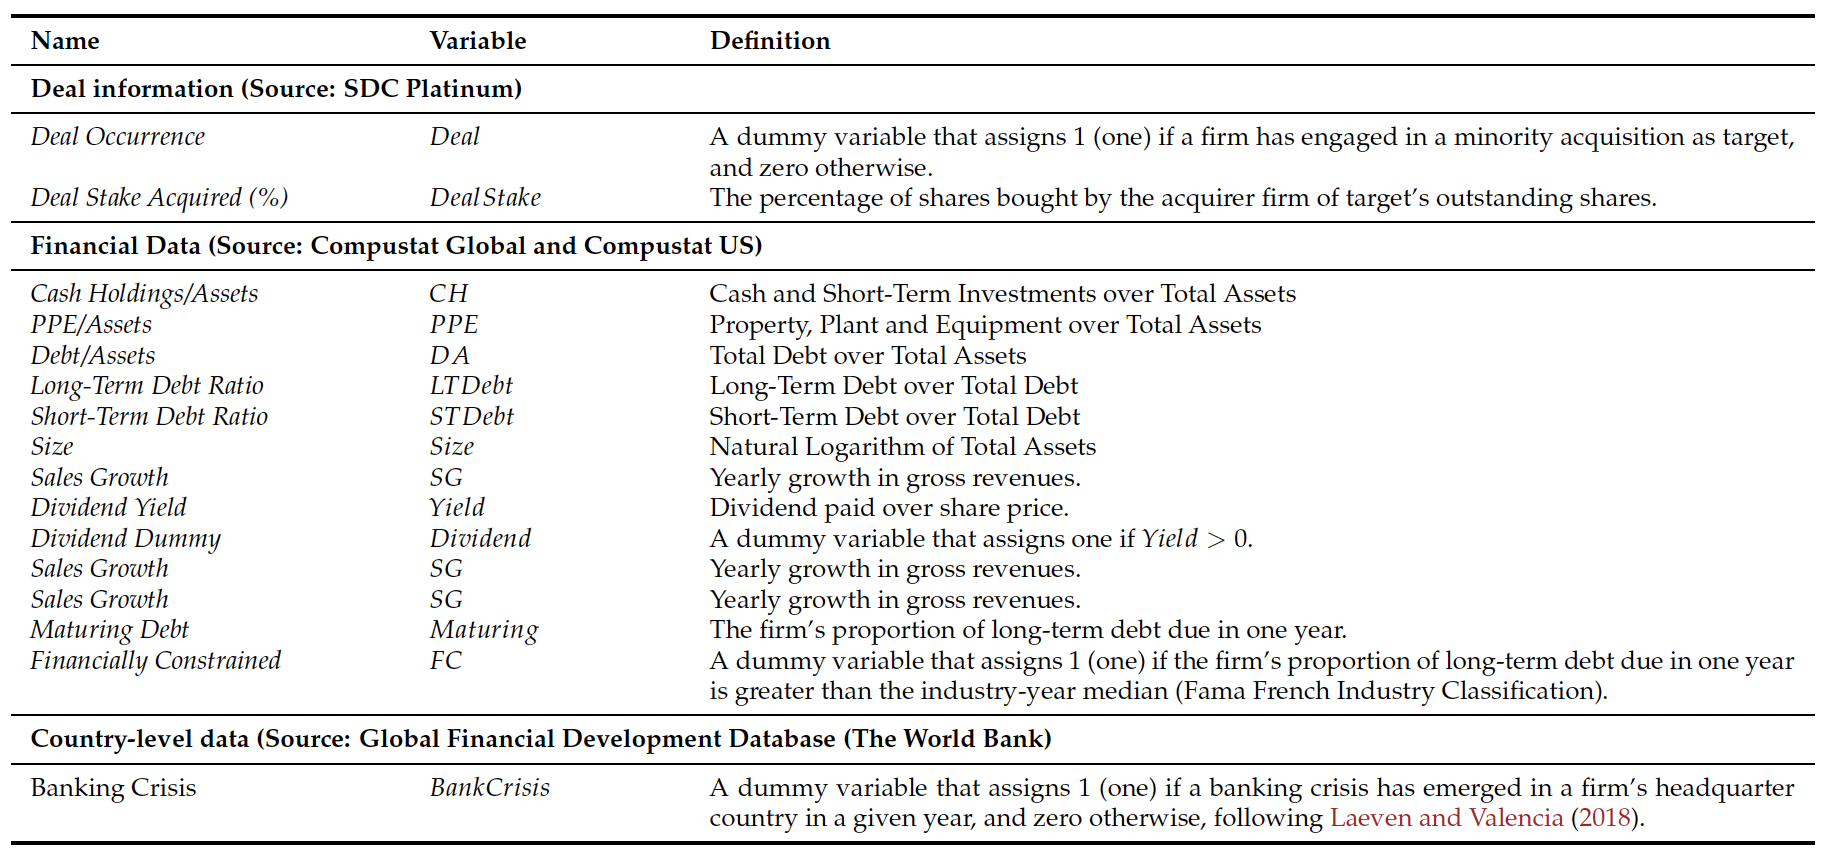
\includegraphics[scale=0.35]{P1/Table 1 - Variables.png}
\end{figure}
%\vspace{-5}
%\hyperlink{P3_Strategy}{\beamerbutton{Back}}
\end{frame}

\begin{frame}{Descriptive Statistics}\label{Table2}
\begin{figure}
\centering
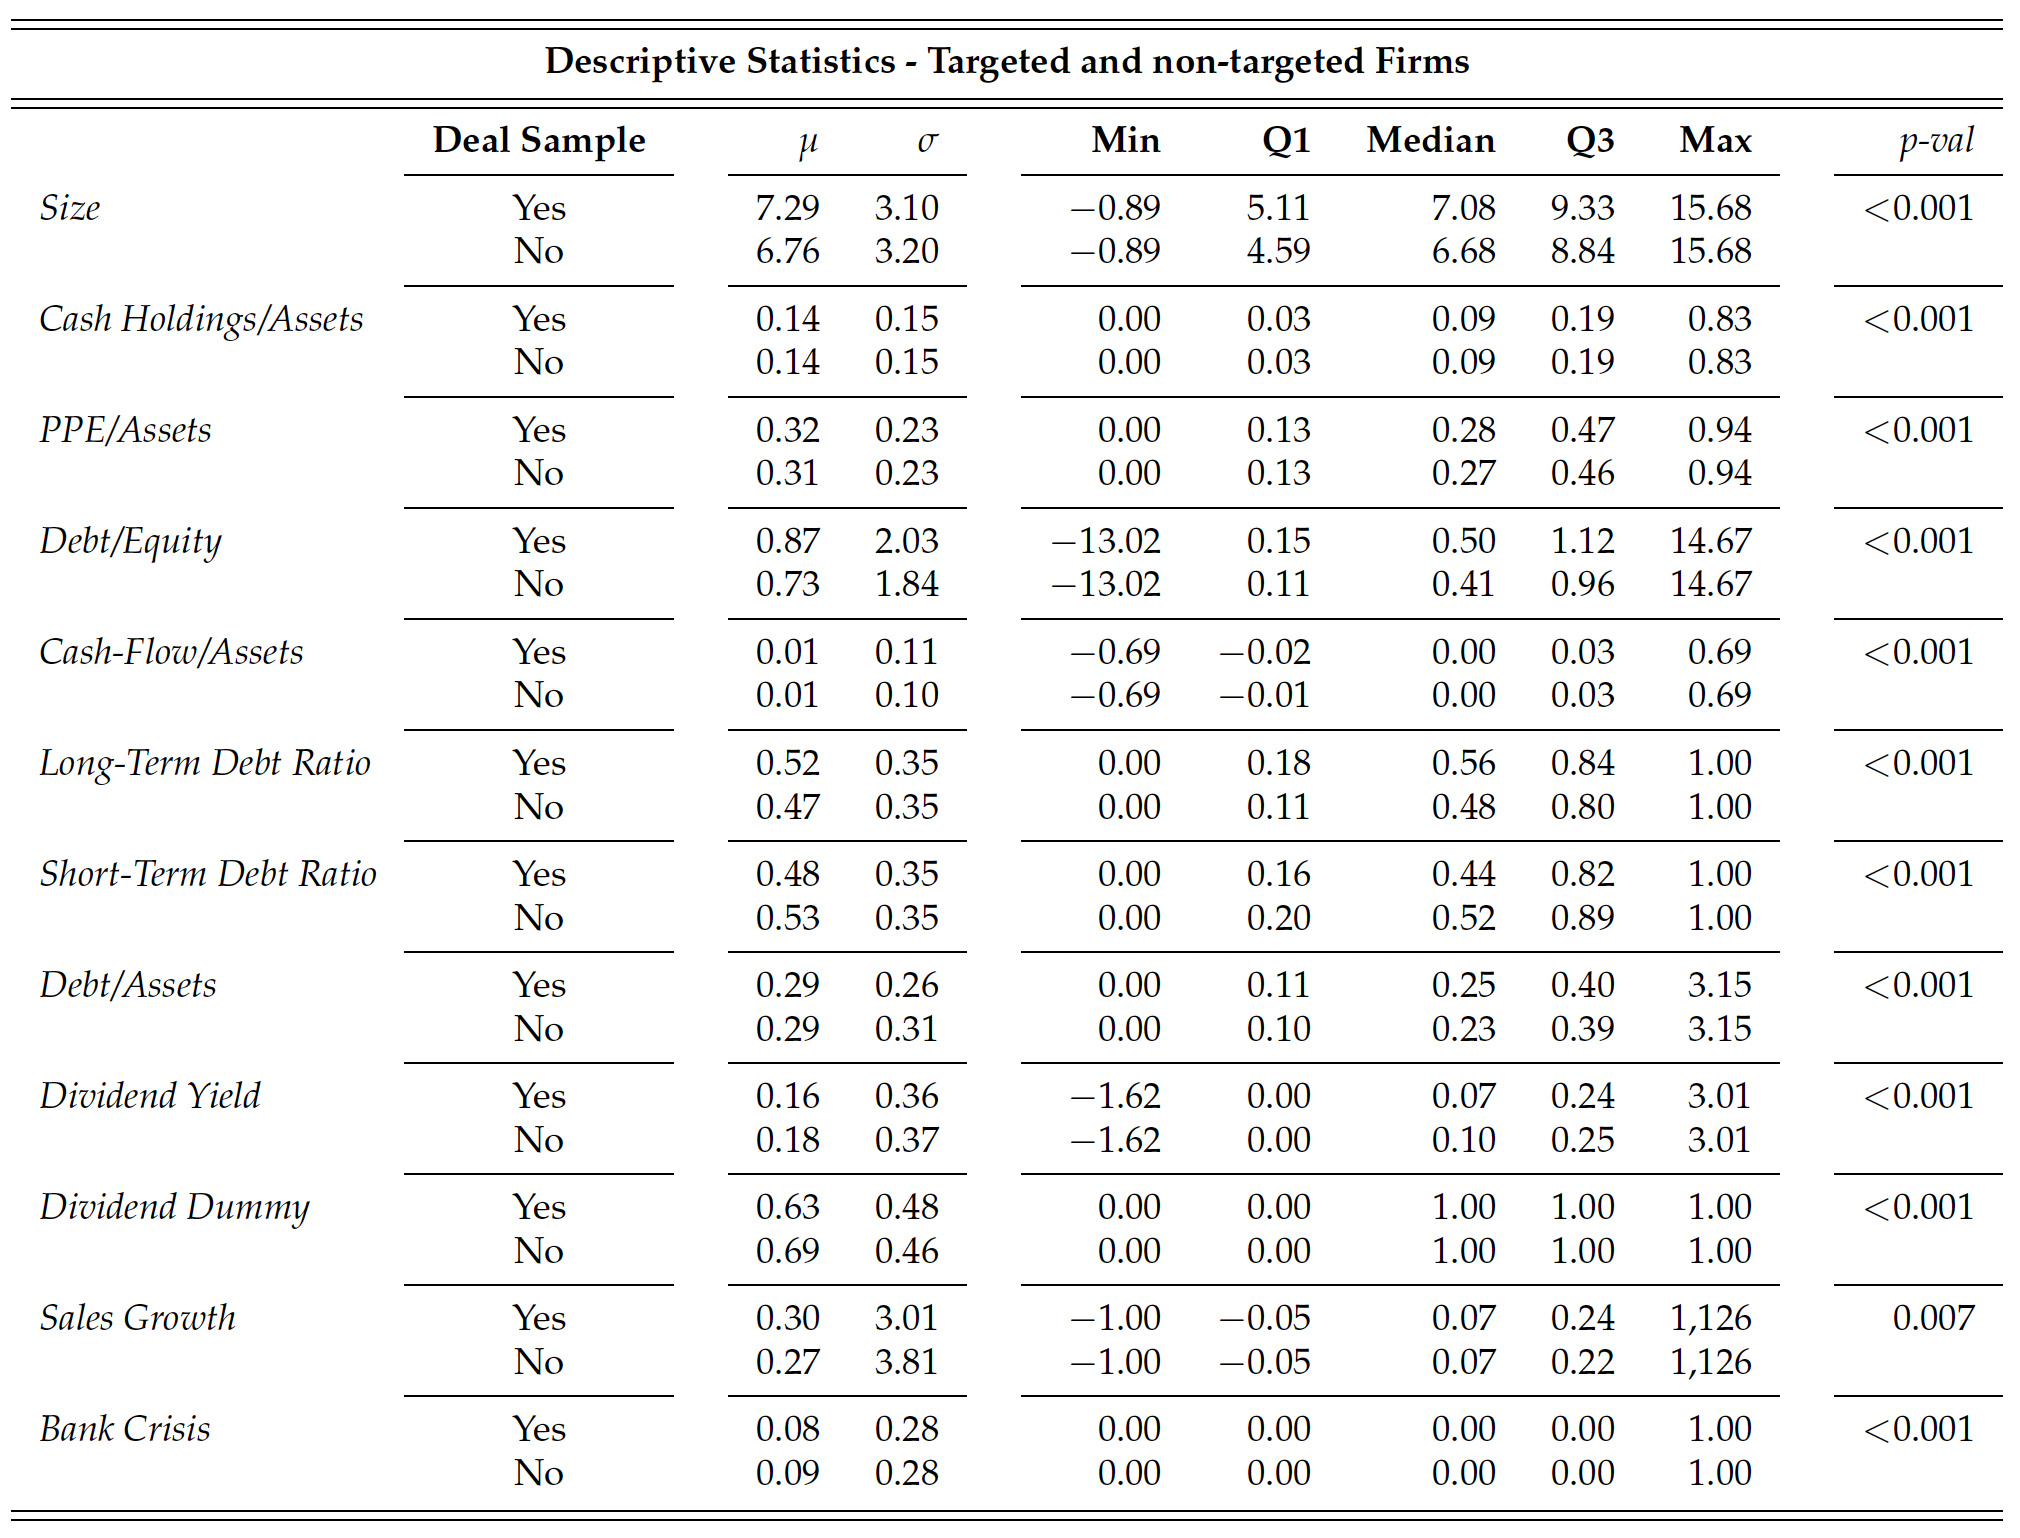
\includegraphics[scale=0.3]{P1/Table 2 - Descriptive Statistics.png}
\end{figure}
%\vspace{-5}
%\hyperlink{P3_Strategy}{\beamerbutton{Back}}
\end{frame}

\begin{frame}{\#1: Firms exposed to a liquidity shock during a banking crisis are more likely to engage in M\&A transactions}\label{P11}

% Table created by stargazer v.5.2.2 by Marek Hlavac, Harvard University. E-mail: hlavac at fas.harvard.edu
% Date and time: seg, set 27, 2021 - 17:26:10
\begin{table}[!htbp] \centering 
\scalebox{0.65}{
\begin{tabular}{@{\extracolsep{5pt}}lcccc} 
\\[-1.8ex]\hline 
\hline \\[-1.8ex] 
 & \multicolumn{4}{c}{Deal Dummy (1 if Deal in that year, zero otherwise)} \\ 
\cline{2-5} 
\\[-1.8ex] & \multicolumn{4}{c}{} \\ 
\\[-1.8ex] & (1) & (2) & (3) & (4)\\ 
\hline \\[-1.8ex] 
 FC & 0.002$^{***}$ & 0.003$^{***}$ & 0.003$^{***}$ & 0.001 \\ 
  & (0.001) & (0.001) & (0.001) & (0.001) \\ 
  & & & & \\ 
 Banking Crisis & $-$0.005$^{***}$ & $-$0.005$^{***}$ & $-$0.012$^{***}$ & $-$0.004$^{**}$ \\ 
  & (0.001) & (0.001) & (0.001) & (0.002) \\ 
  & & & & \\ 
 \textcolor{blue}{FC x Banking Crisis} & \textcolor{blue}{0.004$^{**}$} & \textcolor{blue}{0.004$^{*}$} & \textcolor{blue}{0.006$^{***}$} & \textcolor{blue}{0.005$^{**}$} \\ 
  & (0.002) & (0.002) & (0.002) & (0.002) \\ 
  & & & & \\ 
\hline \\[-1.8ex] 
Controls? & No & Yes & Yes & Yes \\ 
Year fixed effects & No & Yes & Yes & Yes \\ 
Firm fixed effects & No & No & Yes & Yes \\ 
Controls x Crisis? & No & No & No & Yes \\ 
S.E Clustering & Firm & Firm & Firm & Firm \\ 
Observations & 601,784 & 504,815 & 504,815 & 504,815 \\ 
R$^{2}$ & 0.0001 & 0.0003 & 0.002 & 0.086 \\ 
\hline 
\hline \\[-1.8ex] 
\textit{Note:}  & \multicolumn{4}{r}{$^{*}$p$<$0.1; $^{**}$p$<$0.05; $^{***}$p$<$0.01} \\ 
\end{tabular}}
\end{table} 

\end{frame}

\begin{frame}{\#2: Robustness check - Different sets of controls}\label{P11a}
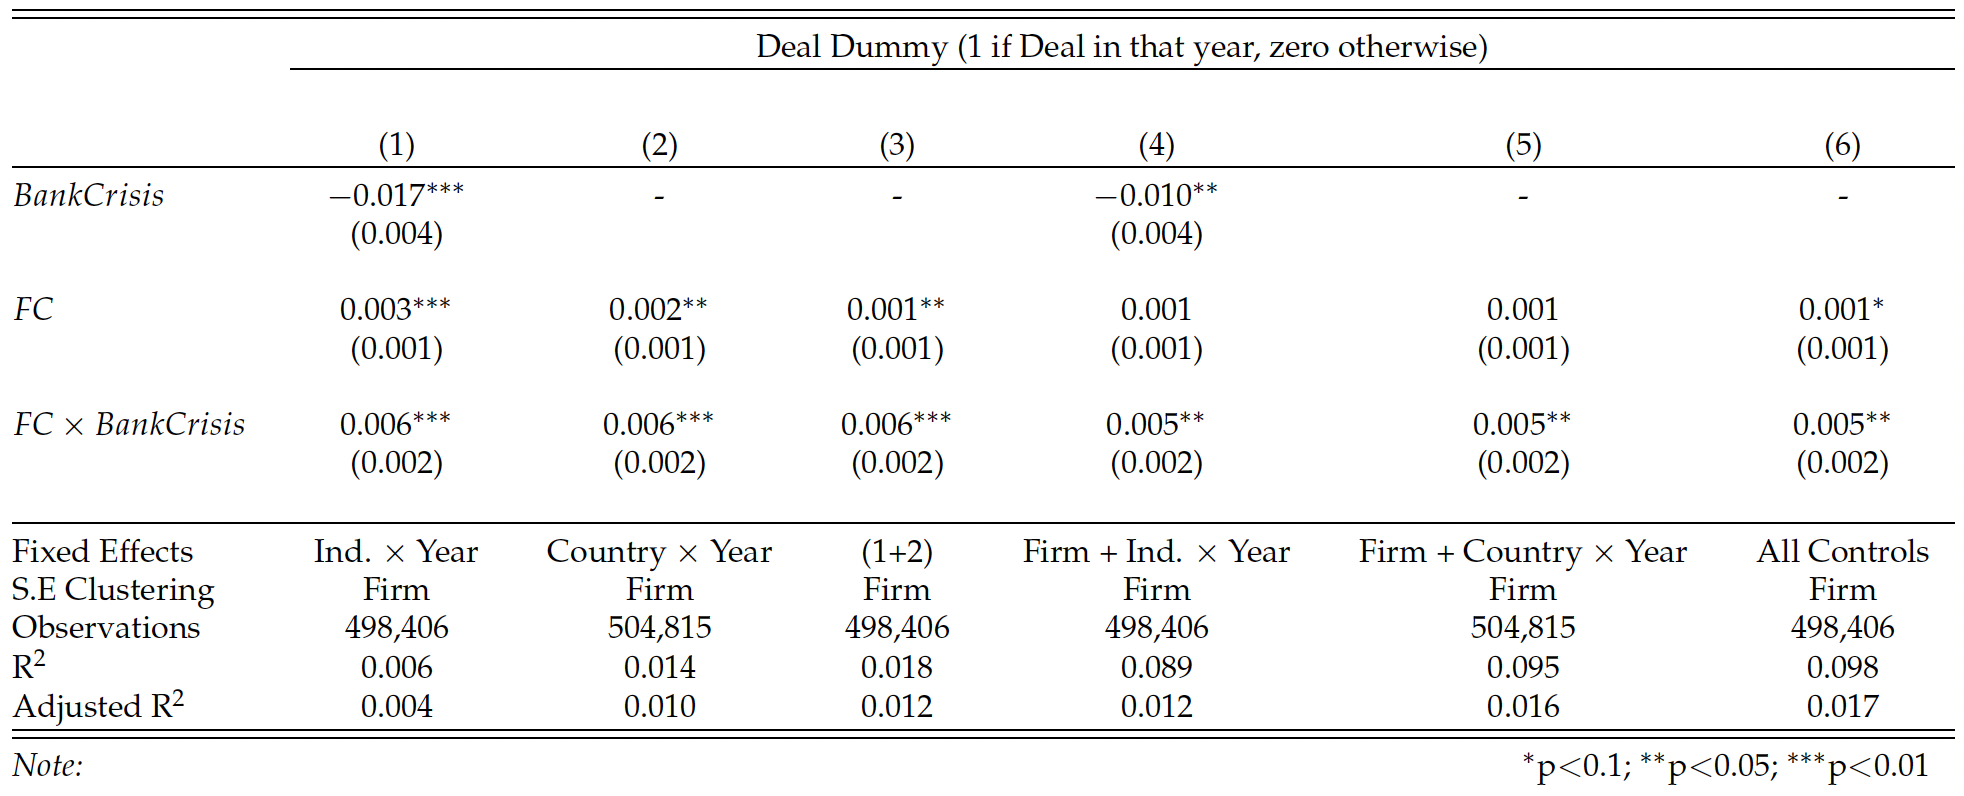
\includegraphics[scale=0.35]{P1/Table 4 - Robustness 1.png}
\end{frame}

\begin{frame}{\#3a: Robustness check - Deal likelihood around banking crisis (Table)}\label{P11a}
\centering
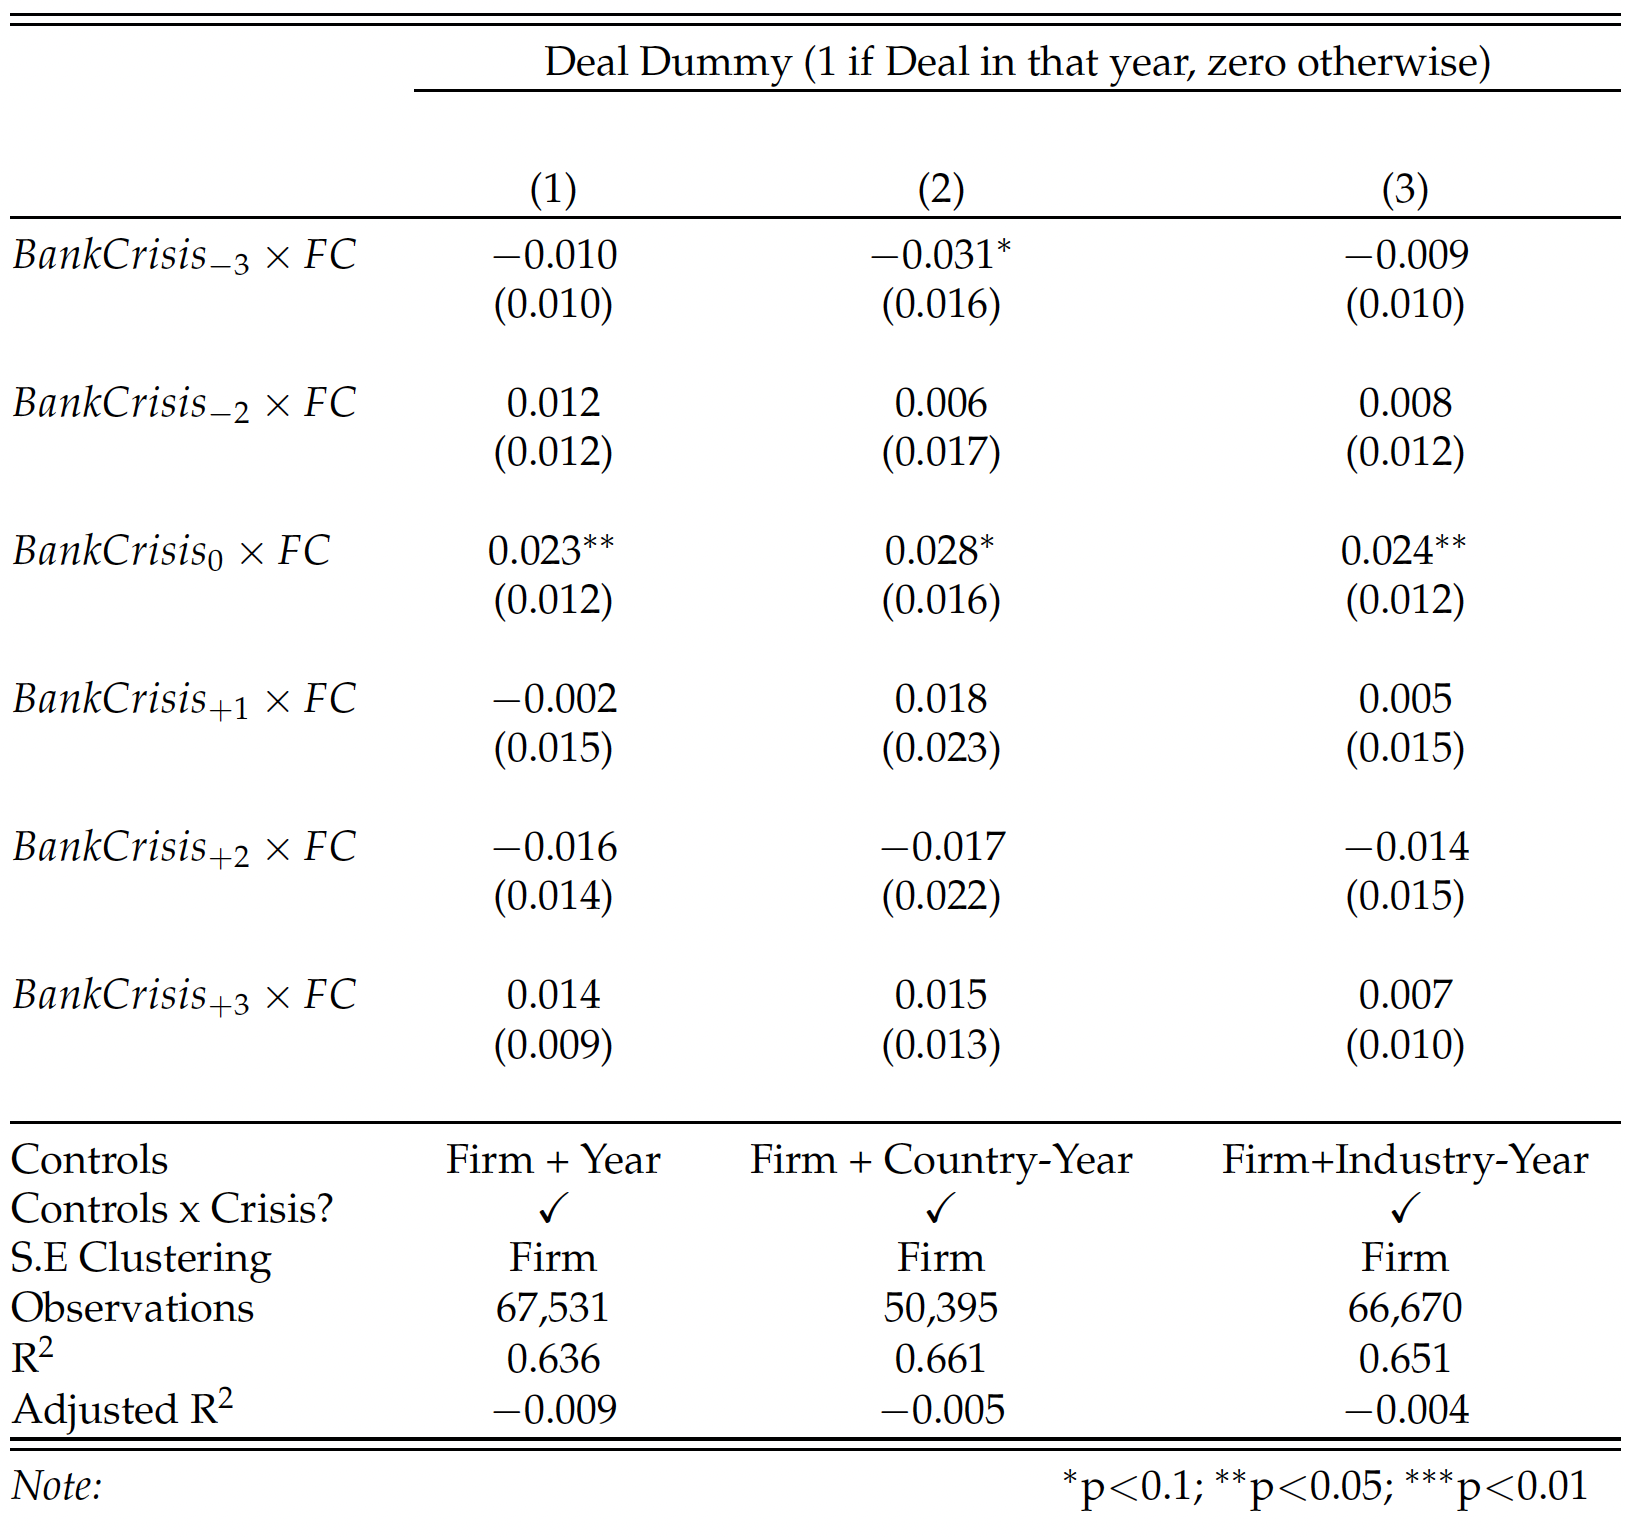
\includegraphics[scale=0.25]{P1/Table 5 - Robustness 2.png}
\end{frame}

\begin{frame}{\#3b: Robustness check - Deal likelihood around banking crisis (Graph)}\label{P11b}
\centering
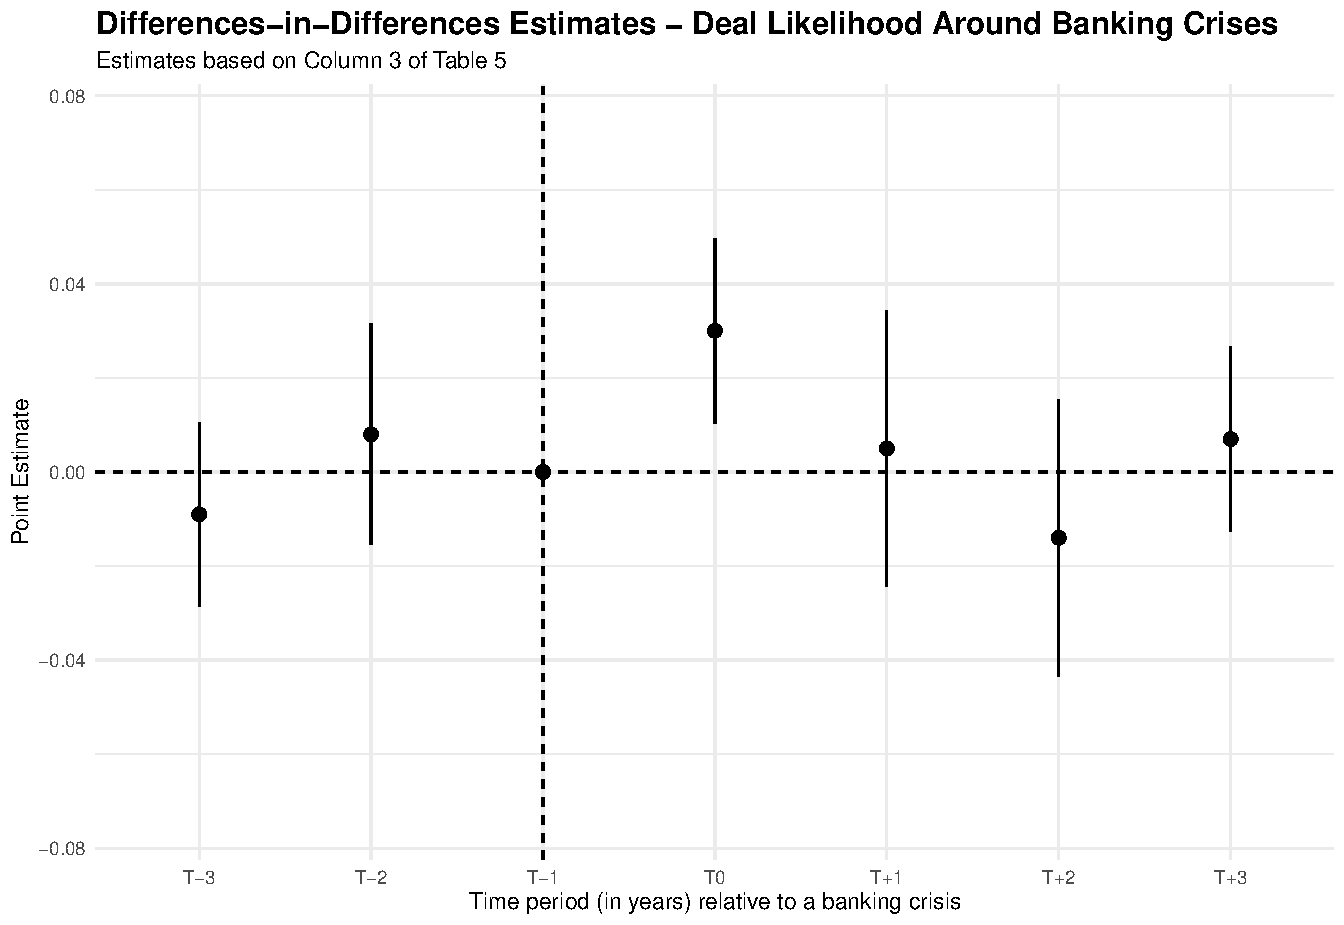
\includegraphics[scale=0.45]{P1/Dynamic DD.pdf}
\end{frame}


\begin{frame}{\#4a: \textit{Ex-post} effects in firms exposed to liquidity constraints}\label{P12}
\begin{figure}
    \centering
    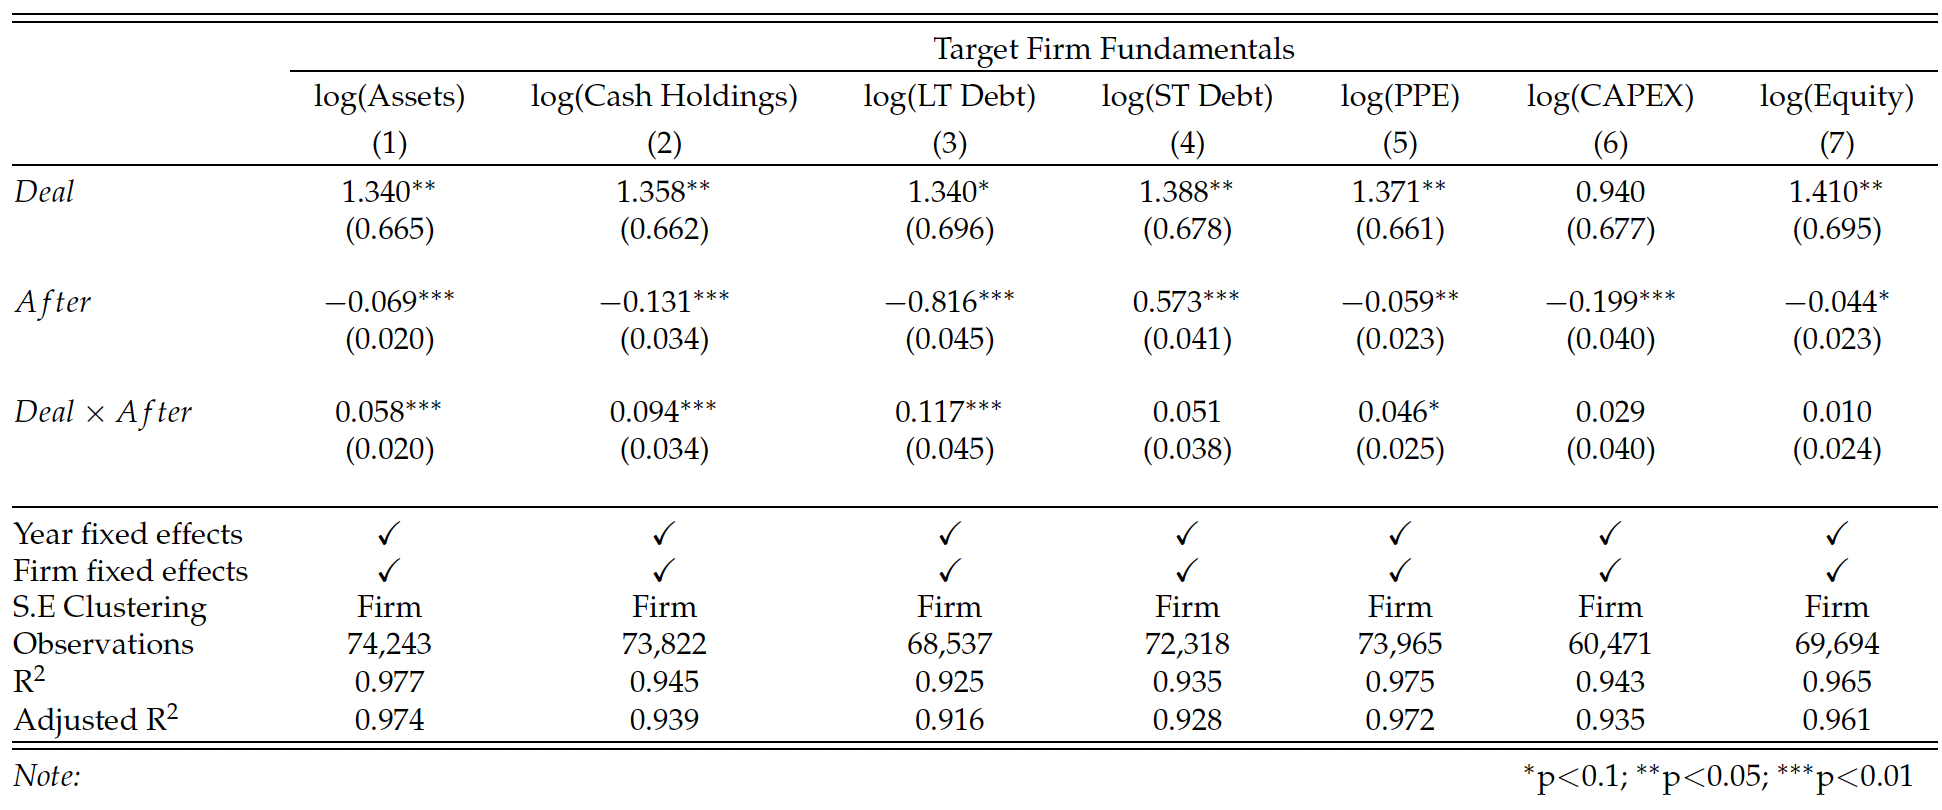
\includegraphics[scale=0.35]{P1/Table 6 - Ex-post effects.png}
\end{figure}
\end{frame}

\begin{frame}{\#4b: \textit{Ex-post} effects: The increase in total assets is primarily driven by increases in cash holdings and PPE}
\begin{figure}
    \centering
    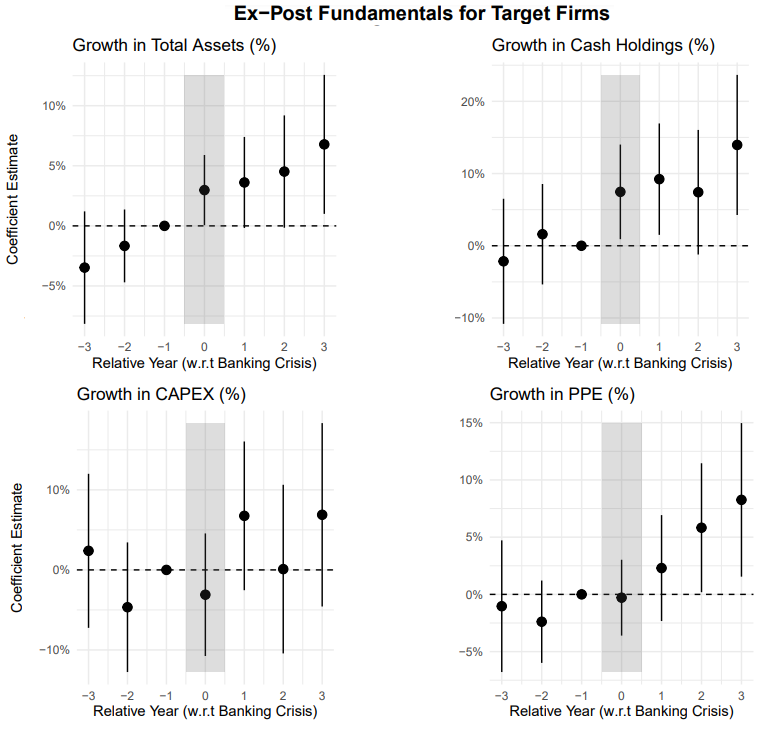
\includegraphics[scale=0.35]{P1/Dynamic Panel1.png}
\end{figure}
\end{frame}

\begin{frame}{\#4c: \textit{Ex-post} effects: The changes in corporate finance is primarily driven by changes in long-term debt}
\begin{figure}
    \centering
    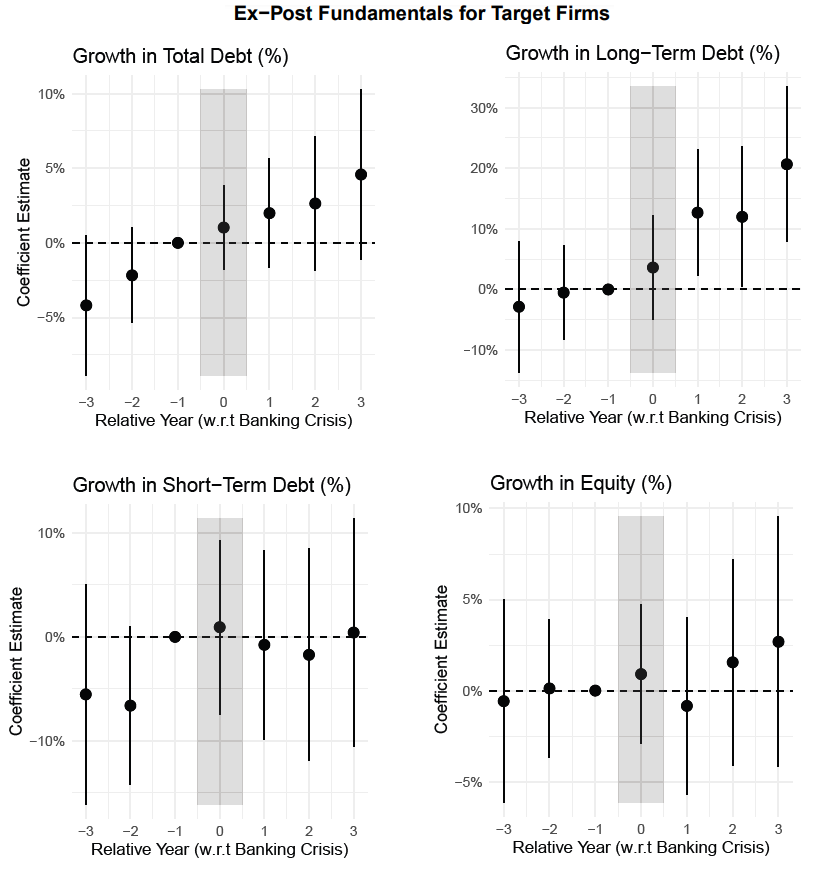
\includegraphics[scale=0.3]{P1/Dynamic Panel2.png}
\end{figure}
\end{frame}

\begin{frame}{\#4d: \textit{Ex-post} effects in firms not exposed to liquidity constraints.}
\begin{figure}
    \centering
    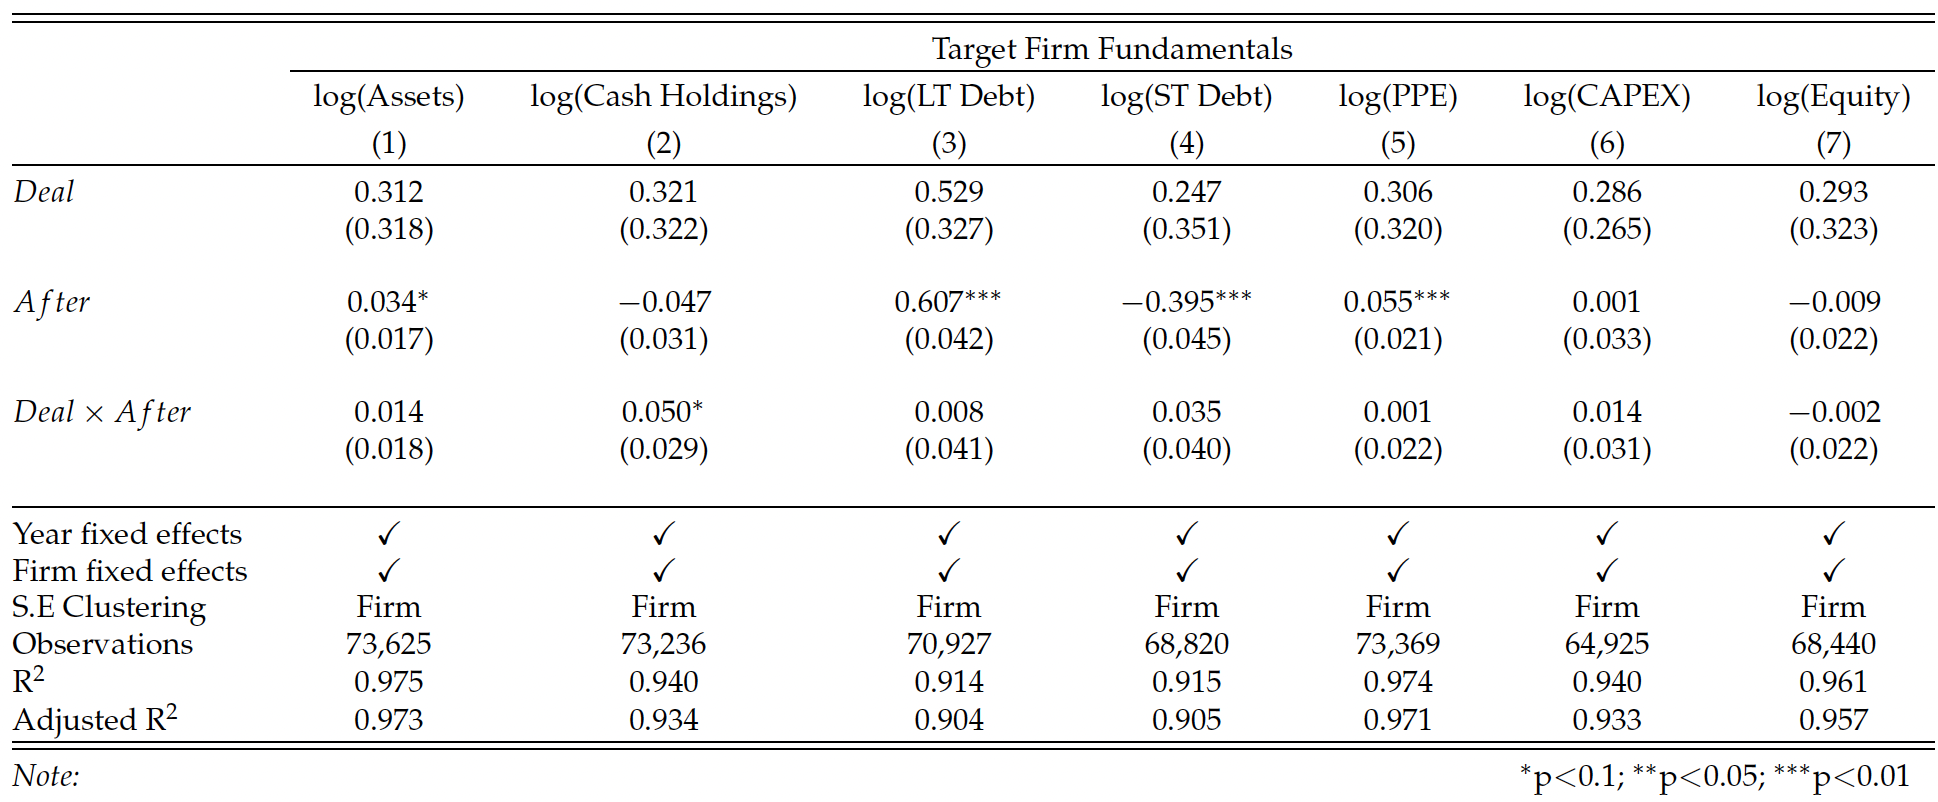
\includegraphics[scale=0.35]{P1/Table 7 - Ex-post effects unconstrained firms.png}
\end{figure}
\end{frame}

\begin{comment}
\begin{frame}{\#4e: \textit{Ex-post} effects in firms not exposed to liquidity constraints.}
\begin{figure}
    \centering
    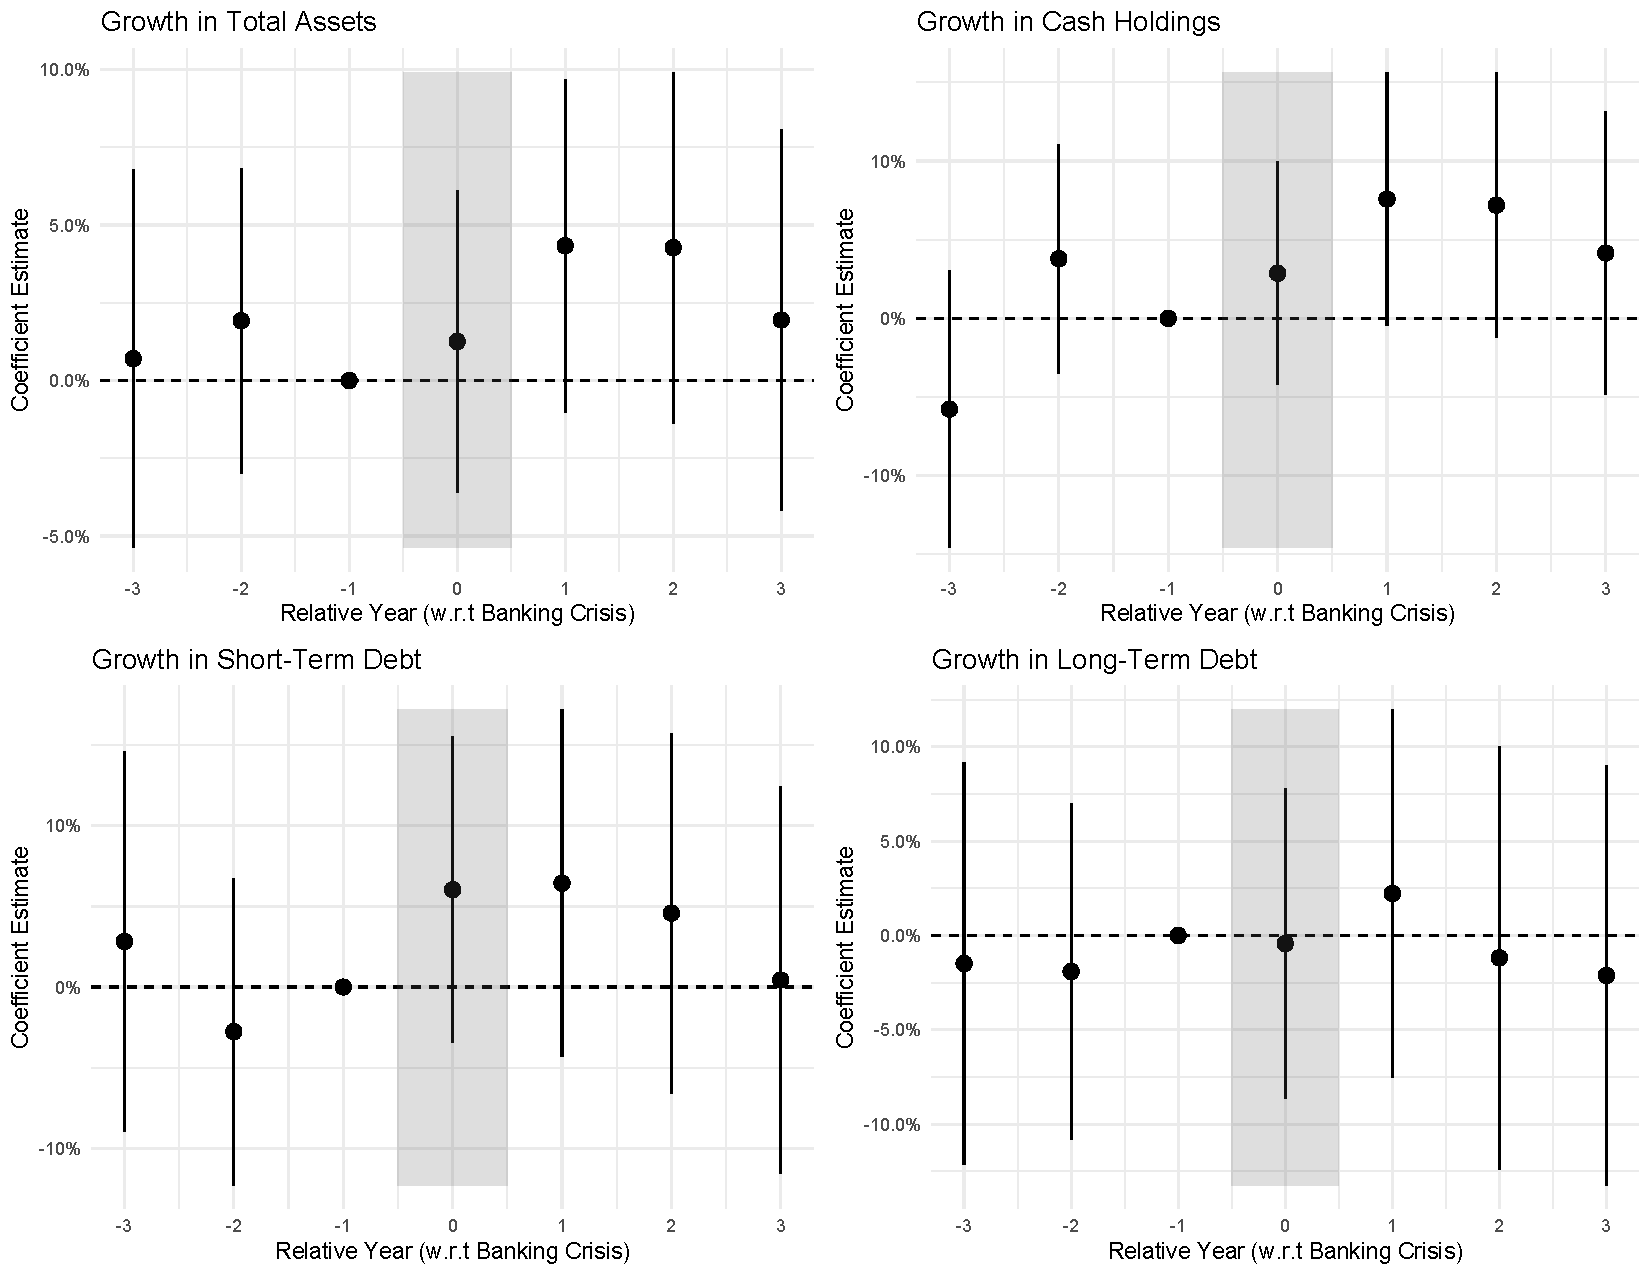
\includegraphics[scale=0.35]{P1/ExPost Dynamics False.pdf}
\end{figure}
%\hyperlink{P1_Results}{\beamerbutton{Back}}
\end{frame}
\end{comment}

\begin{frame}{\#5: Data on debt and equity issuance-level shows that \textit{ex-post} changes are driven by \textbf{debt}, and not equity, issuance}\label{P11c}

% Table created by stargazer v.5.2.3 by Marek Hlavac, Social Policy Institute. E-mail: marek.hlavac at gmail.com
% Date and time: Sat, Feb 25, 2023 - 3:01:49 PM
\begin{table}[!htbp] \centering
  \label{DebtReg}
  \scalebox{0.7}{
\begin{tabular}{@{\extracolsep{5pt}}lcccc} 
\\[-1.8ex]\hline 
\hline \\[-1.8ex] 
 & \multicolumn{4}{c}{\textit{Dependent variable:}} \\ 
\cline{2-5} 
\\[-1.8ex] & \multicolumn{3}{c}{log(1+Issuance)} & log(1+Maturity) \\ 
\\[-1.8ex] & \textbf{Full Sample} & Debt & Equity & Debt\\ 
\\[-1.8ex] & (1) & (2) & (3) & (4)\\ 
\hline \\[-1.8ex] 
 $FC$ & \textbf{$-$0.128$^{**}$} & $-$0.272$^{***}$ & 0.062 & 0.0002 \\ 
  & (0.057) & (0.083) & (0.070) & (0.030) \\ 
  & & & & \\ 
 $After$ & \textbf{$-$0.078} & $-$4.821$^{***}$ & $-$1.029$^{**}$ & 0.123 \\ 
  & (0.403) & (0.446) & (0.411) & (0.133) \\ 
  & & & & \\ 
 \textcolor{blue}{\textbf{$FC \times After$}} &  \textcolor{blue}{\textbf{0.188}$^{***}$} &  \textcolor{blue}{0.248$^{**}$} &  0.026 &  $-$0.005 \\ 
  & (0.071) & (0.110) & (0.089) & (0.038) \\ 
  & & & & \\ 
\hline \\[-1.8ex] 
Controls & \checkmark & \checkmark & \checkmark & \checkmark \\ 
Year x Industry FE & \checkmark & \checkmark & \checkmark & \checkmark \\ 
Year x Target Country FE & \checkmark & \checkmark & \checkmark & \checkmark \\ 
Deal fixed FE & \checkmark & \checkmark & \checkmark & \checkmark \\ 
Controls $\times$ Crisis & \checkmark & \checkmark & \checkmark & \checkmark \\ 
S.E Clustering & Deal & Deal & Deal & Deal \\ 
Observations & 45,537 & 19,109 & 26,428 & 18,257 \\ 
R$^{2}$ & 0.554 & 0.651 & 0.580 & 0.577 \\ 
\hline 
\hline \\[-1.8ex] 
\textit{Note:}  & \multicolumn{4}{r}{$^{*}$p$<$0.1; $^{**}$p$<$0.05; $^{***}$p$<$0.01} \\ 
\end{tabular}}
\end{table} 

\vspace{3mm}
\end{frame}

\begin{frame}{\#6: From where did the money flow? The target firms accessed markets characterized by high issuance volume.}\label{P11e}


% Table created by stargazer v.5.2.3 by Marek Hlavac, Social Policy Institute. E-mail: marek.hlavac at gmail.com
% Date and time: Sat, Feb 25, 2023 - 3:29:45 PM
\begin{table}[!htbp] \centering 
  \label{tab:DebtRegCountry} 

   \scalebox{0.5}{
\begin{tabular}{@{\extracolsep{5pt}}lcccc} 
\\[-1.8ex]\hline 
\hline \\[-1.8ex] 
 & \multicolumn{4}{c}{\textit{Dependent variable:}} \\ 
\cline{2-5} 
\\[-1.8ex] & \multicolumn{4}{c}{log(1+Issuance)} \\ 
\\[-1.8ex] & \textbf{Low-High} & High-High & Low-Low & High-Low\\ 
\\[-1.8ex] & (1) & (2) & (3) & (4)\\ 
\hline \\[-1.8ex] 
 $FC$ & \textbf{$-$0.788$^{***}$} & $-$0.055 & 0.121 & 0.802$^{***}$ \\ 
  & (0.288) & (0.065) & (0.084) & (0.255) \\ 
  & & & & \\ 
 $After$ & \textbf{2.925$^{***}$} & 0.096 & - & - \\ 
  & (0.753) & (0.512) & (0.000) & (0.000) \\ 
  & & & & \\ 
\textcolor{blue}{\textbf{$FC \times After$}} & \textcolor{blue}{\textbf{0.451}$^{**}$} & 0.096 & $-$0.125 & $-$0.839$^{***}$ \\ 
  & (0.227) & (0.079) & (0.145) & (0.315) \\ 
  & & & & \\ 
\hline \\[-1.8ex] 
Controls & \checkmark & \checkmark & \checkmark & \checkmark \\ 
Year x Industry FE & \checkmark & \checkmark & \checkmark & \checkmark \\ 
Year x Target Country FE & \checkmark & \checkmark & \checkmark & \checkmark \\ 
Deal FE & \checkmark & \checkmark & \checkmark & \checkmark \\ 
Controls $\times$ Crisis & \checkmark & \checkmark & \checkmark & \checkmark \\ 
S.E Clustering & Deal & Deal & Deal & Deal \\ 
Sample & Q1 & Q2 & Q3 & Q4 \\ 
Observations & 4,218 & 29,392 & 5,569 & 6,358 \\ 
R$^{2}$ & 0.702 & 0.616 & 0.739 & 0.364 \\ 
Adjusted R$^{2}$ & 0.591 & 0.519 & 0.600 & 0.225 \\ 
\hline 
\hline \\[-1.8ex] 
\textit{Note:}  & \multicolumn{4}{r}{$^{*}$p$<$0.1; $^{**}$p$<$0.05; $^{***}$p$<$0.01} \\ 
\end{tabular}} 
\end{table} 

\begin{itemize}
\item \textbf{Low-High} indicates that the target firm is not headquartered in one of the top 10 countries with the highest debt issuance volume, yet it issues in a country that is within this top 10 group.

\end{itemize}
\end{frame}

\begin{frame}{Other Robustness Checks}\label{P1_Results}

\begin{itemize}

%\item No significant \textit{ex-post} effects for $FC_{i,t}=0$.
    
\item \textbf{Better-informed firms?} Effects are higher for cross-border acquisitions.         

\item  \textbf{Industry-specific acquisitions}? Effects are higher when the acquirer is a financial firm.

\item \textbf{A change of control?} Effects are driven by \textit{minority} acquisitions, and increasing on the size of the equity stake

\item \textbf{Driven by selection?} Comparing only target firms during banking crises 

\end{itemize}
\vspace{3mm}

\textbf{Robustness Checks:} \hyperlink{P13}{\beamerbutton{Go}}
\vspace{3mm}

%We contribute to prior literature by highlighting a channel by which firms can circumvent the effects of credit supply shortfalls.

\end{frame}




\begin{frame}{Effects are higher for cross-border acquisitions}\label{P13}

% Table created by stargazer v.5.2.2 by Marek Hlavac, Harvard University. E-mail: hlavac at fas.harvard.edu
% Date and time: ter, set 28, 2021 - 20:34:31
\begin{table}[!htbp] \centering 
\scalebox{0.45}{
\begin{tabular}{@{\extracolsep{5pt}}lcccccccccc} 
\\[-1.8ex]\hline 
\hline \\[-1.8ex] 
 & \multicolumn{10}{c}{\textit{Dependent variable:}} \\ 
\cline{2-11} 
\\[-1.8ex] & \multicolumn{2}{c}{log(Assets)} & \multicolumn{2}{c}{log(Cash Holdings)} & \multicolumn{2}{c}{log(Long-Term Debt)} & \multicolumn{2}{c}{log(Short-Term Debt)} & \multicolumn{2}{c}{log(Total Debt)} \\ 
\\[-1.8ex] & (1) & (2) & (3) & (4) & (5) & (6) & (7) & (8) & (9) & (10)\\ 
\hline \\[-1.8ex] 
 Deal x After & \textcolor{blue}{0.126$^{***}$} & 0.038$^{**}$ & \textcolor{blue}{0.119$^{***}$} & 0.049$^{**}$ & \textcolor{blue}{0.185$^{***}$} & 0.066$^{*}$ & \textcolor{blue}{0.172$^{***}$} & 0.104$^{***}$ & \textcolor{blue}{0.127$^{***}$} & 0.026$^{*}$ \\ 
  & (0.020) & (0.016) & (0.026) & (0.021) & (0.047) & (0.037) & (0.034) & (0.025) & (0.019) & (0.014) \\ 
  & & & & & & & & & & \\ 
\hline \\[-1.8ex] 
Sample & Cross-border & Domestic & Cross-border & Domestic & Cross-border & Domestic & Cross-border & Domestic & Cross-border & Domestic \\ 
Year fixed effects & Yes & Yes & Yes & Yes & Yes & Yes & Yes & Yes & Yes & Yes \\ 
Firm fixed effects & Yes & Yes & Yes & Yes & Yes & Yes & Yes & Yes & Yes & Yes \\ 
S.E Clustering & Firm & Firm & Firm & Firm & Firm & Firm & Firm & Firm & Firm & Firm \\ 
Observations & 34,230 & 58,040 & 34,230 & 58,040 & 34,230 & 58,040 & 34,230 & 58,040 & 34,225 & 58,035 \\ 
R$^{2}$ & 0.976 & 0.979 & 0.956 & 0.958 & 0.899 & 0.907 & 0.933 & 0.940 & 0.977 & 0.981 \\ 
Adjusted R$^{2}$ & 0.971 & 0.975 & 0.947 & 0.950 & 0.878 & 0.888 & 0.920 & 0.928 & 0.973 & 0.977 \\ 

\hline 
\hline \\[-1.8ex] 
\textit{Note:}  & \multicolumn{10}{r}{$^{*}$p$<$0.1; $^{**}$p$<$0.05; $^{***}$p$<$0.01} \\ 
\end{tabular}}
\end{table} 

\hyperlink{P1_Results}{\beamerbutton{Back}}
\end{frame}

\begin{frame}{Effects are higher when the acquirer is a financial firm}\label{P13}

% Table created by stargazer v.5.2.2 by Marek Hlavac, Harvard University. E-mail: hlavac at fas.harvard.edu
% Date and time: qua, set 29, 2021 - 09:49:48
\begin{table}[!htbp] \centering 
\scalebox{0.45}{
\begin{tabular}{@{\extracolsep{5pt}}lcccccccccc} 
\\[-1.8ex]\hline 
\hline \\[-1.8ex] 
 & \multicolumn{10}{c}{\textit{Dependent variable:}} \\ 
\cline{2-11} 
\\[-1.8ex] & \multicolumn{2}{c}{log(Assets)} & \multicolumn{2}{c}{log(Cash Holdings)} & \multicolumn{2}{c}{log(Long-Term Debt)} & \multicolumn{2}{c}{log(Short-Term Debt)} & \multicolumn{2}{c}{log(Total Debt)} \\ 
\\[-1.8ex] & (1) & (2) & (3) & (4) & (5) & (6) & (7) & (8) & (9) & (10)\\ 
\hline \\[-1.8ex] 
 Deal x After & 0.061$^{**}$ & \textcolor{blue}{0.100$^{***}$} & 0.058$^{*}$ & \textcolor{blue}{0.115$^{***}$} & 0.066 & \textcolor{blue}{0.161$^{***}$} & 0.136$^{***}$ & \textcolor{blue}{0.153$^{***}$} & 0.054$^{**}$ & \textcolor{blue}{0.093$^{***}$} \\ 
  & (0.024) & (0.028) & (0.032) & (0.036) & (0.053) & (0.054) & (0.039) & (0.041) & (0.023) & (0.027) \\ 
  & & & & & & & & & & \\ 
\hline \\[-1.8ex] 
Sample & Non-Financial & Financial & Non-Financial & Financial & Non-Financial & Financial & Non-Financial & Financial & Non-Financial & Financial \\ 
Year fixed effects & Yes & Yes & Yes & Yes & Yes & Yes & Yes & Yes & Yes & Yes \\ 
Firm fixed effects & Yes & Yes & Yes & Yes & Yes & Yes & Yes & Yes & Yes & Yes \\ 
S.E Clustering & Firm & Firm & Firm & Firm & Firm & Firm & Firm & Firm & Firm & Firm \\ 
Observations & 42,001 & 50,269 & 42,001 & 50,269 & 42,001 & 50,269 & 42,001 & 50,269 & 41,996 & 50,264 \\ 
R$^{2}$ & 0.977 & 0.977 & 0.958 & 0.955 & 0.903 & 0.903 & 0.937 & 0.936 & 0.978 & 0.978 \\ 
Adjusted R$^{2}$ & 0.973 & 0.974 & 0.951 & 0.949 & 0.887 & 0.890 & 0.927 & 0.927 & 0.975 & 0.975 \\ 
\hline 
\hline \\[-1.8ex] 
\textit{Note:}  & \multicolumn{10}{r}{$^{*}$p$<$0.1; $^{**}$p$<$0.05; $^{***}$p$<$0.01} \\ 
\end{tabular}}
\end{table} 

\hyperlink{P1_Results}{\beamerbutton{Back}}
\end{frame}

\begin{frame}{A change of control? Effects are driven by \textit{minority acquisitions}...}\label{P13}

% Table created by stargazer v.5.2.2 by Marek Hlavac, Harvard University. E-mail: hlavac at fas.harvard.edu
% Date and time: qua, set 29, 2021 - 10:17:50
\begin{table}[!htbp] \centering
\scalebox{0.5}{
\begin{tabular}{@{\extracolsep{5pt}}lcccccccccc} 
\\[-1.8ex]\hline 
\hline \\[-1.8ex] 
 & \multicolumn{10}{c}{\textit{Dependent variable:}} \\ 
\cline{2-11} 
\\[-1.8ex] & \multicolumn{2}{c}{log(Assets)} & \multicolumn{2}{c}{log(Cash Holdings)} & \multicolumn{2}{c}{log(Long-Term Debt)} & \multicolumn{2}{c}{log(Short-Term Debt)} & \multicolumn{2}{c}{log(Total Debt)} \\ 
\\[-1.8ex] & (1) & (2) & (3) & (4) & (5) & (6) & (7) & (8) & (9) & (10)\\ 
\hline \\[-1.8ex] 
 Deal x After & \textcolor{blue}{0.091$^{***}$} & 0.060$^{***}$ & \textcolor{blue}{0.116$^{***}$} & 0.043 & \textcolor{blue}{0.192$^{***}$} & $-$0.006 & \textcolor{blue}{0.176$^{***}$} & 0.062$^{*}$ & \textcolor{blue}{0.097$^{***}$} & 0.029 \\ 
  & (0.028) & (0.023) & (0.038) & (0.028) & (0.057) & (0.047) & (0.043) & (0.035) & (0.028) & (0.021) \\ 
  & & & & & & & & & & \\ 
\hline \\[-1.8ex] 
Sample & Minority & Majority & Minority & Majority & Minority & Majority & Minority & Majority & Minority & Majority \\ 
Year fixed effects & Yes & Yes & Yes & Yes & Yes & Yes & Yes & Yes & Yes & Yes \\ 
Firm fixed effects & Yes & Yes & Yes & Yes & Yes & Yes & Yes & Yes & Yes & Yes \\ 
S.E Clustering & Firm & Firm & Firm & Firm & Firm & Firm & Firm & Firm & Firm & Firm \\ 
Observations & 52,639 & 35,832 & 52,639 & 35,832 & 52,639 & 35,832 & 52,639 & 35,832 & 52,633 & 35,828 \\ 
R$^{2}$ & 0.976 & 0.977 & 0.954 & 0.960 & 0.901 & 0.901 & 0.935 & 0.939 & 0.977 & 0.979 \\ 
Adjusted R$^{2}$ & 0.973 & 0.973 & 0.948 & 0.953 & 0.889 & 0.883 & 0.926 & 0.928 & 0.974 & 0.975 \\ 
\hline 
\hline \\[-1.8ex] 
\textit{Note:}  & \multicolumn{10}{r}{$^{*}$p$<$0.1; $^{**}$p$<$0.05; $^{***}$p$<$0.01} \\ 
\end{tabular}}
\caption{\textit{Ex-Post} Effects - Minority and Majority Acquisitions} 
\end{table} 

\hyperlink{P1_Results}{\beamerbutton{Back}}
\end{frame}

\begin{frame}{...but increase on the size of the equity stake}\label{P13}
\centering
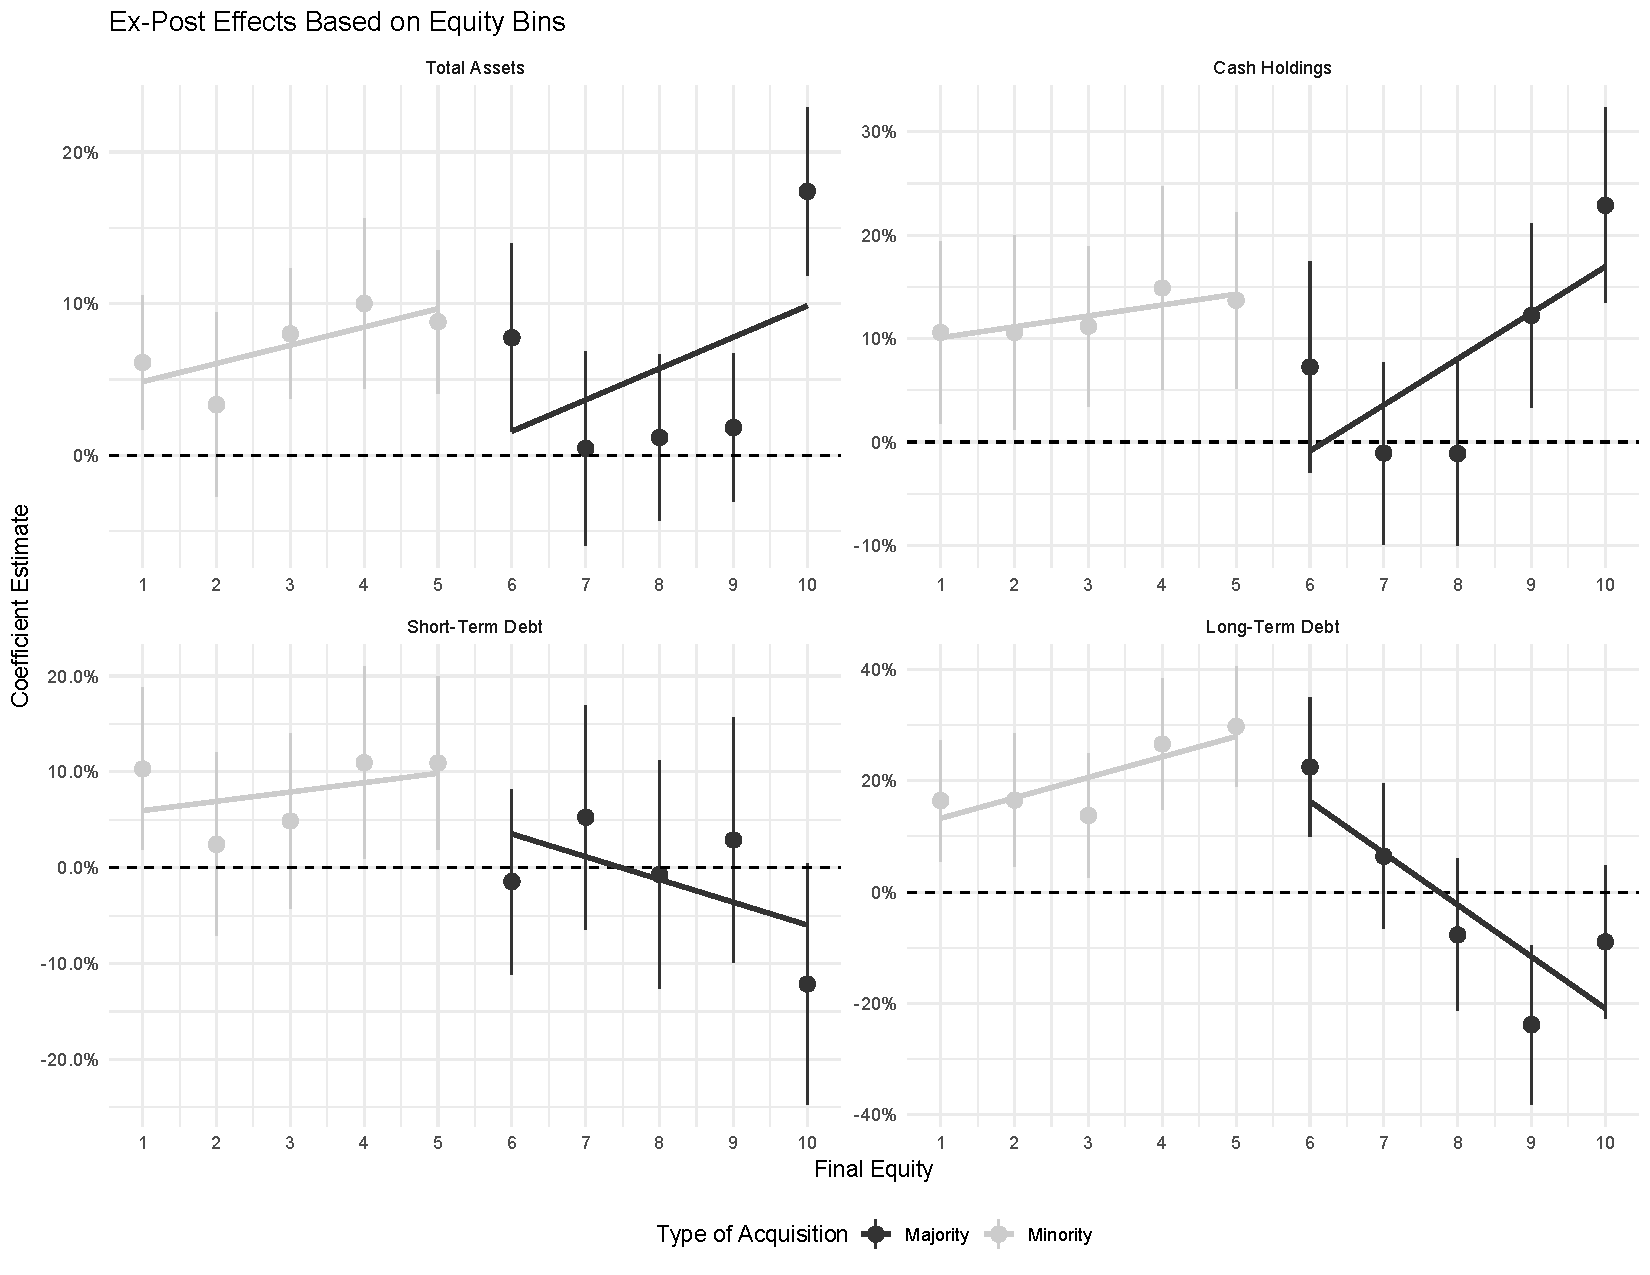
\includegraphics[scale=0.32]{P1/Equity_Bins.pdf}
\hyperlink{P1_Results}{\beamerbutton{Back}}
\end{frame}

\begin{frame}{conditional on being targeted, effects are present only for the sample of firms with maturing debt}\label{P13}

% Table created by stargazer v.5.2.2 by Marek Hlavac, Harvard University. E-mail: hlavac at fas.harvard.edu
% Date and time: sex, out 08, 2021 - 10:22:05
\begin{table}[!htbp] \centering 
  \label{} 
  \scalebox{0.65}{
\begin{tabular}{@{\extracolsep{5pt}}lccccc} 
\\[-1.8ex]\hline 
\hline \\[-1.8ex] 
 & \multicolumn{5}{c}{\textit{Ex-post} effects} \\ 
\cline{2-6} 
\\[-1.8ex] & log(Assets) & log(Cash Holdings) & log(Total Debt) & log(CAPEX) & log(PPE) \\ 
\\[-1.8ex] & (1) & (2) & (3) & (4) & (5)\\ 
\hline \\[-1.8ex] 
 FC & $-$0.107 & $-$0.134 & $-$0.227$^{***}$ & $-$0.157$^{*}$ & $-$0.134$^{*}$ \\ 
  & (0.066) & (0.120) & (0.076) & (0.083) & (0.070) \\ 
  & & & & & \\ 
 After & $-$0.066 & $-$0.103 & 0.045 & $-$0.419$^{***}$ & $-$0.057 \\ 
  & (0.123) & (0.139) & (0.136) & (0.144) & (0.131) \\ 
  & & & & & \\ 
 FC x After & 0.084 & 0.119 & 0.173$^{*}$ & $-$0.041 & 0.072 \\ 
  & (0.086) & (0.120) & (0.093) & (0.100) & (0.088) \\ 
  & & & & & \\ 
\hline \\[-1.8ex] 
Year fixed effects & Yes & Yes & Yes & Yes & Yes \\ 
Firm fixed effects & Yes & Yes & Yes & Yes & Yes \\ 
S.E Clustering & Firm & Firm & Firm & Firm & Firm  \\ 
Observations & 8,197 & 8,162 & 8,197 & 7,745 & 8,184 \\ 
R$^{2}$ & 0.907 & 0.866 & 0.902 & 0.892 & 0.913 \\ 
Adjusted R$^{2}$ & 0.900 & 0.855 & 0.894 & 0.883 & 0.906 \\ 
\hline 
\hline \\[-1.8ex] 
\textit{Note:}  & \multicolumn{5}{r}{$^{*}$p$<$0.1; $^{**}$p$<$0.05; $^{***}$p$<$0.01} \\ 
\end{tabular}} 
  \caption{Ex-Post Effects - Considering only the Deal Subsample during Banking Crises} 
\end{table} 

\hyperlink{P1_Results}{\beamerbutton{Back}}
\end{frame}

\begin{frame}{What do our results tell about liquidity?}

\begin{itemize}
    \item Results so far show evidence in favor of
    \begin{enumerate}
        \item increased deal likelihood for liquidity-constrained firms; and
        \item increased \textit{ex-post} growth after credit supply shocks for those that have been acquired. 
    \end{enumerate}
    
    \item Can we assert that the channel that generates these two predictions is \textbf{liquidity-related}, and not related to other channels of M\&A outcomes?
    
    \item Auxiliary results show that our results are unlikely to be driven by other channels discussed in the M\&A literature:
    \begin{enumerate}
    
        \item \textbf{Better-informed firms?} Effects are driven by cross-border acquisitions. 
        
        \item  \textbf{Industry-specific acquisitions}? Effects are higher when the acquirer is a financial firm. 
        
        \item \textbf{A change of control?} Minority \textit{vis-a-vis} majority acquisitions. 
        
        \item \textbf{Skin in the game?} Final equity stake held by the acquirer. 
        
        \item \textbf{Driven by selection?} Comparing only target firms during banking crises.       
    \end{enumerate}

\end{itemize}

\end{frame}

\begin{frame}{Conclusion}

We investigate the interplay between M\&As and financial constraints during periods of credit supply shocks.

\begin{enumerate}
\item Our results show that firms with maturing debt in times of banking crises are more likely to engage in M\&A transactions to relieve liquidity constraints.
    
\item \textit{Ex-post} results show that these firms are able to attenuate potential liquidity issues—firms that engage in M\&A transactions invest more and raise more debt than their peers.

\end{enumerate}

\textbf{These \textit{ex-post} effects are mainly driven by:}
\begin{enumerate}
        \item Cross-border acquisitions
        \item Minority acquisitions
        \item Financial acquirers %and same industry (at the 4-Digit)
        \end{enumerate}
It seems that the \textbf{certification effect} is the prevailing mechanism explaining our results.
\end{frame}


\begin{frame}{}

    \huge Thank you \& Questions\\
        \\~\\
%    \normalsize \textbf{Our contacts}\\
%    Lucas Macoris <lucasmacoris@gmail.com> \& \\
%    Luiz Ricardo Kabbach <lkabbach@unav.es>
    
\end{frame}

\end{document}